\documentclass[../main.tex]{subfiles}
\subsection{DAC}
DAC or the Digital to Analog Converter is used to generate analogue signals based on the digital values it receives.
The DAC is connected to the 3.5mm headphone jack.
Initialising the DAC for inputs is quite simple.
Within the \emph{setup.c} file there is the \emph{setupDAC} function.

\begin{minted}{objdump}
    *CMU_HFPERCLKEN0    |=  1 << 17;
    *DAC0_CTRL          =   0x50010;
    *DAC0_CH0CTRL       =   1;
    *DAC0_CH1CTRL       =   1;
\end{minted}

This sets the DAC to get inputs from the \emph{DAC0\_CH0DATA} and the \emph{DAC0\_CH1DATA} registers.
As this continuous stream of data is converted to a analogue signal by the DAC, a sound waves would be generated from the speakers connected to the jack.

\begin{figure}
    \centering
    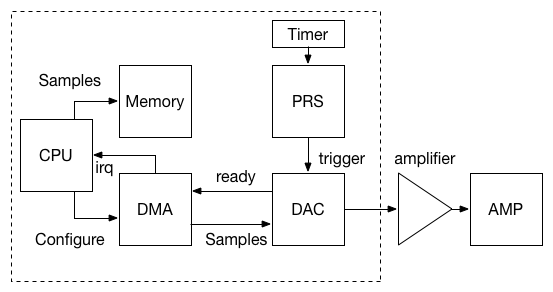
\includegraphics[width=0.4\textwidth]{fig/DMA-DAC.png}
    \caption{Overview of DMA-DAC system}
    \label{fig:DMA-DAC}
\end{figure}

